\chapter{PETSc-Optimization} % (fold)
\label{cha:petsc}

The PETSc solver is the core of our simulation. It is responsible for actually
solving the equation system, which makes it the most time-consuming part of
running a simulation. However, it has a lot of options which could speed it up.

%%%%%%%%%%%%%%%%%%%%%

When optimizing our PETSc solver we tried multiple combinations of
preconditioned and solver for the global and local grids. Some combinations
showed a lot of promise with execution times up to 5 times faster than the
original solver. We selected the top 3 of these options with the most promise
and ran a scaling test, which quickly showed that the optimizations were not
always consistently better. Nevertheless, we performed strong scaling tests over
laminar and algebraically turbulent simulations on grids of cell size 256x64 and
512x128. The resulting plots can be found below. Left, the total poison solve
time has been plotted for all 3 variants tested along with the default
configuration, while right the speedup relative to the default configurations
has been plotted. One can extract that the execution time of the poison solver
is highly dependent the number of process, and therefore the domain
decomposition of the problem.

In general no pattern could be found to be constant, but often one of the
preconditioned variant of the fgmres-asm-preonly-ilu f proved to be faster than
the default configuration.

While scaling with algebraic turbulence models, the default configuration was
shown to be more consistent, but nevertheless, optimized solvers showed
performance in some cases. In the laminar case, although the default
configuration proved itself as stable, it was constantly beat by one of the
tested solver pre-conditioner combinations as can be seen below.  This
especially was true for jobs with 32 ranks or more.

Note: Some runs took longer than the allotted 30-minute execution time, and
therefore have no data plot for those runs. The data has never the less been
interpolated across the entire domain.

Side note: Another puzzling discovery was that the order of the conditioners and
pre- conditioners in the the petsc comandline arg script seemed to have a large
influence on PETSc's performance, at times in a drastically negative way. A
simple rearrangement of the petsc comandlind arg file quickly remedied this
issue, but as of this point, no logical reason for this is known to us.

\section{Approach}

Actually PETSc has so many options that you cannot conceivably test them
all. You can select solvers and preconditioners for the problem and when you are
working in parallel, you can also choose a different pair of solver and
preconditioner for the subdomains. If you want to go really deep, you can even
make this choice on a subdomain by subdomain basis, so that you could, for
example, use a different solver near the boundary than in the middle of a
channel scenario. On top of this there there are specific options for certain
solvers and preconditioners for fine-tuning. In view of this fact, we chose to
try an automatic approach.

\section{Preselection}

We initially hoped that a lot of the options would take continuous values. We
had the idea that we could interpret the run time of a simulation as a function
$f(p) : \mathbb{R}^{n} \rightarrow \mathbb{R}$ and use a numerical optimization
algorithm to find a configuration for minimal run time. Though the options
turned out to be mostly of the discrete variety which foiled our plan and made
this an integer optimization problem.

To combat the combinatoric explosion of option combinations, we decided to split
the optimization into two phases. In a first step we only try combinations of
solvers and preconditioners without changing specific options from their default
values because we suspect that that these have the most impact on run time over
all.

Tables \ref{fig:petsc-opt-combinations-1x1} until
\ref{fig:petsc-opt-combinations-16x4} show the resulting Poisson solving time
for all combinations of solver, preconditioner, subdomain solver and subdomain
preconditioner in a channel scenario of dimensions $5 \times 1$ with an
increasingly fine grid. The tables are of different length, because we filtered
out combinations that either diverged or did not finish in time.

Based on this ranking we chose the combination of a BiConjugate Gradient Squared
(\texttt{bcgs}) solver with an Additive Schwarz (\texttt{asm}) preconditioner on
the whole domain level and an NOP (\texttt{preonly}) solver with an incomplete
LU (\texttt{ilu}) preconditioner for further investigation because that
combination gave consistently very good results, time-wise as well as
simulation-wise. Some of the other fast combinations produced simulation
results.

\begin{table}[h]
  \tiny
  \centering
  \begin{tabular}{cccccc}
    \hline Rank & Solver & Preconditioner & Sub-Solver & Sub-Preconditioner & PETSc-Time\\ \hline

    1 & bcgs & ilu & - & - & 2.50662 \\
    2 & bcgs & jacobi & - & - & 3.85583 \\
    3 & gcr & ilu & - & - & 15.7704 \\
    4 & bcgs & bjacobi & - & - & 17.835 \\
    5 & fgmres & asm & - & - & 40.7862 \\
    6 & fgmres & gasm & - & - & 41.7788 \\
    7 & fgmres & jacobi & - & - & 47.3308 \\
    8 & gcr & asm & - & - & 49.5737 \\
    9 & gcr & gasm & - & - & 50.6497 \\
    10 & bcgs & gasm & - & - & 57.9513 \\
    11 & dgmres & asm & - & - & 75.0263 \\
    12 & gmres & gasm & - & - & 75.0506 \\
    13 & dgmres & gasm & - & - & 75.1658 \\
    14 & bcgs & bddc & - & - & 136.995 \\
    15 & cg & bddc & - & - & 137.031 \\
    16 & fgmres & bddc & - & - & 137.057 \\
    17 & dgmres & bddc & - & - & 137.127 \\
    18 & tcqmr & bddc & - & - & 137.148 \\
    19 & cr & bddc & - & - & 137.156 \\
    20 & chebyshev & bddc & - & - & 137.67 \\
    21 & bicg & bddc & - & - & 137.983 \\
    22 & lsqr & bddc & - & - & 138.319 \\
    \hline
  \end{tabular}
  \caption{PETSc-times of a $1 \times 1$ decomposition on a $128 \times 32$ grid in a $5 \times 1$ channel scenario}
  \label{fig:petsc-opt-combinations-1x1}
\end{table}

\begin{table}[h]
  \tiny
  \centering
  \begin{tabular}{cccccc}
    \hline Rank & Solver & Preconditioner & Sub-Solver & Sub-Preconditioner & PETSc-Time\\ \hline

    1 & bcgs & bjacobi & preonly & ilu & 9.91897 \\
    2 & bcgs & bjacobi & preonly & bjacobi & 10.2778 \\
    3 & bcgs & bjacobi & preonly & asm & 11.0625 \\
    4 & bcgs & asm & preonly & bjacobi & 12.0636 \\
    5 & bcgs & asm & preonly & ilu & 12.0825 \\
    6 & bcgs & jacobi & bcgs & asm & 16.8702 \\
    7 & bcgs & jacobi & bcgs & bjacobi & 16.8819 \\
    8 & bcgs & asm & preonly & jacobi & 21.4934 \\
    9 & fgmres & asm & preonly & ilu & 25.0637 \\
    10 & fgmres & bjacobi & preonly & asm & 26.5028 \\
    11 & gcr & bjacobi & preonly & ilu & 48.7232 \\
    12 & gcr & bjacobi & preonly & asm & 52.4674 \\
    13 & gcr & bjacobi & preonly & gasm & 54.3274 \\
    14 & fgmres & asm & preonly & asm & 69.0118 \\
    15 & gcr & asm & preonly & ilu & 77.1786 \\
    16 & gcr & asm & preonly & asm & 80.9108 \\
    17 & fgmres & jacobi & fgmres & asm & 86.4742 \\
    18 & fgmres & jacobi & fgmres & ilu & 86.9231 \\
    19 & fgmres & jacobi & fgmres & gasm & 88.5556 \\
    20 & fgmres & bjacobi & preonly & jacobi & 92.1365 \\
    21 & gcr & jacobi & preonly & asm & 114.156 \\
    22 & fgmres & asm & fgmres & asm & 174.54 \\
    23 & fgmres & asm & fgmres & gasm & 175.754 \\
    24 & gmres & asm & gmres & gasm & 261.226 \\
    25 & fgmres & jacobi & preonly & asm & 273.189 \\
    26 & fgmres & jacobi & fgmres & jacobi & 273.44 \\
    27 & fgmres & jacobi & preonly & gasm & 273.533 \\
    28 & gcr & jacobi & gcr & gasm & 322.474 \\
    29 & gcr & jacobi & gcr & ilu & 322.506 \\
    \hline
  \end{tabular}
  \caption{PETSc-times of a $4 \times 1$ decomposition on a $256 \times 64$ grid in a $5 \times 1$ channel scenario}
  \label{fig:petsc-opt-combinations-4x1}
\end{table}

\begin{table}[h]
  \tiny
  \centering
  \begin{tabular}{cccccc}
    \hline Rank & Solver & Preconditioner & Sub-Solver & Sub-Preconditioner & PETSc-Time\\ \hline

    1 & bcgs & asm & preonly & ilu & 4.84988 \\
    2 & bcgs & asm & preonly & asm & 5.50919 \\
    3 & bcgs & asm & preonly & bjacobi & 5.58179 \\
    4 & bcgs & bjacobi & preonly & gasm & 7.36192 \\
    5 & bcgs & jacobi & preonly & jacobi & 11.5107 \\
    6 & bcgs & jacobi & bcgs & bjacobi & 11.5891 \\
    7 & bcgs & asm & preonly & gasm & 15.0381 \\
    8 & bcgs & jacobi & preonly & bjacobi & 17.6565 \\
    9 & tfqmr & asm & preonly & ilu & 19.7188 \\
    10 & fgmres & bjacobi & preonly & ilu & 22.1083 \\
    11 & gcr & bjacobi & preonly & ilu & 22.3645 \\
    12 & gcr & asm & preonly & ilu & 23.9356 \\
    13 & gcr & asm & preonly & gasm & 24.2038 \\
    14 & gcr & bjacobi & preonly & asm & 24.2789 \\
    15 & bcgs & bjacobi & preonly & ilu & 28.4305 \\
    16 & fgmres & bjacobi & preonly & asm & 29.8764 \\
    17 & bcgs & bjacobi & preonly & bjacobi & 30.8208 \\
    18 & gcr & asm & preonly & asm & 30.8698 \\
    19 & bcgs & bjacobi & preonly & asm & 32.7116 \\
    20 & fgmres & asm & preonly & ilu & 38.1359 \\
    21 & fgmres & asm & preonly & asm & 42.3049 \\
    22 & dgmres & bjacobi & preonly & asm & 43.7851 \\
    23 & bcgs & jacobi & preonly & gasm & 58.8008 \\
    24 & bcgs & jacobi & bcgs & gasm & 59.4479 \\
    25 & fgmres & asm & fgmres & ilu & 62.1746 \\
    26 & fgmres & asm & fgmres & gasm & 70.8113 \\
    27 & dgmres & bjacobi & dgmres & bjacobi & 72.6469 \\
    28 & dgmres & asm & preonly & asm & 74.8014 \\
    29 & bcgs & asm & preonly & jacobi & 84.0214 \\
    30 & fgmres & jacobi & preonly & gasm & 103.675 \\
    31 & fgmres & jacobi & fgmres & ilu & 104.091 \\
    32 & gcr & asm & gcr & asm & 104.336 \\
    33 & fgmres & jacobi & fgmres & gasm & 104.554 \\
    34 & dgmres & bjacobi & preonly & gasm & 105.63 \\
    35 & gcr & asm & preonly & jacobi & 107.927 \\
    36 & gcr & bjacobi & preonly & gasm & 109.618 \\
    37 & bcgs & asm & bcgs & bjacobi & 110.848 \\
    38 & gcr & asm & gcr & gasm & 113.596 \\
    39 & gcr & jacobi & preonly & jacobi & 118.425 \\
    40 & fgmres & jacobi & fgmres & jacobi & 118.499 \\
    41 & gcr & jacobi & preonly & gasm & 118.593 \\
    42 & gcr & jacobi & gcr & jacobi & 118.609 \\
    43 & gcr & jacobi & gcr & ilu & 118.88 \\
    44 & gcr & jacobi & gcr & asm & 120.336 \\
    45 & fgmres & bjacobi & fgmres & ilu & 133.844 \\
    46 & gcr & jacobi & gcr & gasm & 152.573 \\
    47 & dgmres & bjacobi & dgmres & asm & 159.891 \\
    48 & fgmres & jacobi & preonly & jacobi & 167.764 \\
    49 & dgmres & asm & dgmres & bjacobi & 167.945 \\
    50 & fgmres & bjacobi & fgmres & asm & 172.146 \\
    51 & fgmres & bjacobi & fgmres & gasm & 173.781 \\
    52 & gcr & bjacobi & preonly & jacobi & 174.945 \\
    53 & gcr & bjacobi & gcr & gasm & 199.316 \\
    54 & bcgs & asm & bcgs & asm & 203.829 \\
    55 & fgmres & jacobi & preonly & ilu & 208.517 \\
    56 & fgmres & jacobi & preonly & asm & 210.162 \\
    57 & fgmres & asm & preonly & jacobi & 215.341 \\
    58 & fgmres & asm & fgmres & asm & 226.268 \\
    59 & bcgs & bjacobi & bcgs & asm & 227.503 \\
    60 & gcr & bjacobi & gcr & ilu & 230.96 \\
    61 & fgmres & bjacobi & preonly & jacobi & 242.735 \\
    62 & gcr & asm & gcr & ilu & 255.745 \\
    63 & fgmres & asm & fgmres & jacobi & 255.925 \\
    64 & gcr & jacobi & preonly & asm & 265.367 \\
    65 & gcr & jacobi & preonly & ilu & 266.239 \\
    \hline
  \end{tabular}
  \caption{PETSc-times of a $8 \times 2$ decomposition on a $256 \times 64$ grid in a $5 \times 1$ channel scenario}
  \label{fig:petsc-opt-combinations-8x2}
\end{table}

\begin{table}[h]
  \tiny
  \centering
  \begin{tabular}{cccccc}
    \hline Rank & Solver & Preconditioner & Sub-Solver & Sub-Preconditioner & PETSc-Time\\ \hline

    1 & bcgs & asm & preonly & ilu & 8.62323 \\
    2 & bcgs & asm & preonly & gasm & 9.68961 \\
    3 & fgmres & bjacobi & preonly & asm & 31.9078 \\
    4 & gcr & bjacobi & preonly & gasm & 40.1055 \\
    5 & bcgs & bjacobi & preonly & gasm & 41.4188 \\
    6 & fgmres & bjacobi & preonly & gasm & 48.6188 \\
    7 & fgmres & asm & preonly & asm & 50.7413 \\
    8 & bcgs & jacobi & preonly & bjacobi & 53.4876 \\
    9 & gcr & bjacobi & preonly & asm & 57.6915 \\
    10 & bcgs & asm & preonly & jacobi & 74.8086 \\
    11 & dgmres & asm & dgmres & gasm & 89.9251 \\
    12 & fgmres & asm & preonly & gasm & 102.872 \\
    13 & gcr & asm & preonly & asm & 114.781 \\
    14 & dgmres & asm & dgmres & asm & 119.718 \\
    15 & bcgs & jacobi & preonly & gasm & 140.977 \\
    16 & bcgs & bjacobi & preonly & ilu & 159.775 \\
    17 & bcgs & asm & preonly & bjacobi & 169.815 \\
    18 & fgmres & jacobi & fgmres & gasm & 194.687 \\
    19 & fgmres & jacobi & fgmres & jacobi & 196.768 \\
    20 & fgmres & asm & fgmres & asm & 217.465 \\
    21 & fgmres & jacobi & preonly & gasm & 245.402 \\
    22 & fgmres & jacobi & preonly & asm & 268.427 \\
    23 & gcr & asm & gcr & ilu & 272.434 \\
    24 & gcr & asm & gcr & gasm & 278.307 \\
    25 & fgmres & jacobi & preonly & jacobi & 280.382 \\
    26 & gcr & jacobi & gcr & ilu & 384.266 \\
    27 & gcr & asm & preonly & gasm & 391.81 \\
    28 & gcr & jacobi & gcr & gasm & 395.968 \\
    29 & gcr & bjacobi & gcr & gasm & 504.138 \\
    30 & gcr & bjacobi & gcr & asm & 615.469 \\
    31 & fgmres & asm & fgmres & jacobi & 767.893 \\
    32 & fgmres & bjacobi & fgmres & gasm & 817.836 \\
    \hline
  \end{tabular}
  \caption{PETSc-times of a $16 \times 2$ decomposition on a $512 \times 128$ grid in a $5 \times 1$ channel scenario}
  \label{fig:petsc-opt-combinations-16x2}
\end{table}

\begin{table}[h]
  \tiny
  \centering
  \begin{tabular}{cccccc}
    \hline Rank & Solver & Preconditioner & Sub-Solver & Sub-Preconditioner & PETSc-Time\\ \hline

    1 & bcgs & bjacobi & preonly & ilu & 5.50499 \\
    2 & bcgs & asm & preonly & ilu & 6.10181 \\
    3 & bcgs & bjacobi & preonly & bjacobi & 12.1679 \\
    4 & bcgs & jacobi & bcgs & gasm & 28.3655 \\
    5 & bcgs & asm & preonly & bjacobi & 32.8395 \\
    6 & fgmres & bjacobi & preonly & gasm & 41.2223 \\
    7 & gcr & bjacobi & preonly & ilu & 44.5088 \\
    8 & gcr & asm & preonly & asm & 48.7862 \\
    9 & fgmres & asm & preonly & gasm & 53.4382 \\
    10 & gcr & bjacobi & preonly & asm & 56.2883 \\
    11 & fgmres & asm & preonly & asm & 61.2216 \\
    12 & fgmres & bjacobi & preonly & asm & 64.4604 \\
    13 & bcgs & bjacobi & preonly & jacobi & 69.7025 \\
    14 & bcgs & jacobi & bcgs & ilu & 73.5131 \\
    15 & gcr & asm & gcr & asm & 73.723 \\
    16 & bcgs & jacobi & preonly & gasm & 73.7239 \\
    17 & bcgs & jacobi & bcgs & jacobi & 75.3447 \\
    18 & dgmres & asm & dgmres & asm & 88.7668 \\
    19 & gcr & asm & preonly & gasm & 100.861 \\
    20 & bcgs & bjacobi & preonly & gasm & 121.382 \\
    21 & fgmres & asm & fgmres & asm & 126.428 \\
    22 & gcr & bjacobi & preonly & gasm & 145.03 \\
    23 & gcr & asm & gcr & ilu & 177.899 \\
    24 & gcr & jacobi & preonly & asm & 193.614 \\
    25 & fgmres & jacobi & preonly & jacobi & 200.031 \\
    26 & gcr & jacobi & gcr & gasm & 236.216 \\
    27 & dgmres & jacobi & preonly & gasm & 240.373 \\
    28 & gcr & asm & gcr & gasm & 256.96 \\
    29 & fgmres & jacobi & fgmres & gasm & 257.051 \\
    30 & bcgs & asm & bcgs & bjacobi & 274.685 \\
    31 & bcgs & asm & bcgs & gasm & 274.848 \\
    32 & fgmres & jacobi & fgmres & jacobi & 302.701 \\
    33 & fgmres & jacobi & fgmres & asm & 316.879 \\
    34 & gcr & jacobi & preonly & ilu & 323.094 \\
    35 & gcr & asm & preonly & ilu & 324.72 \\
    36 & fgmres & asm & preonly & jacobi & 345.824 \\
    37 & gcr & bjacobi & gcr & ilu & 361.151 \\
    38 & fgmres & asm & fgmres & gasm & 378.469 \\
    39 & bcgs & jacobi & preonly & ilu & 408.646 \\
    40 & fgmres & bjacobi & fgmres & gasm & 421.003 \\
    41 & fgmres & asm & fgmres & jacobi & 442.903 \\
    42 & gcr & bjacobi & gcr & asm & 478.922 \\
    43 & fgmres & bjacobi & preonly & jacobi & 1010.65 \\
    \hline
  \end{tabular}
  \caption{PETSc-times of a $16 \times 4$ decomposition on a $512 \times 128$ grid in a $5 \times 1$ channel scenario}
  \label{fig:petsc-opt-combinations-16x4}
\end{table}

\section{Searching the parameter space}

In a second step we listed all options and their possible values of the chosen
\texttt{bcgs-asm-preonly-ilu} combination. Of these four components only the ilu-preconditioner has any meaningful options. These are
\begin{description}
\item[-pc\_factor\_levels <k>] A natural number from $0$ that describes which
  potence of the matrix should be used to compute the LU decomposition
\item[-pc\_factor\_diagonal\_fill] Always fill in a zero diagonal even if it
  seems unnecesary
\item[-pc\_factor\_reuse\_ordering] Reuse the ordering of the factorized matrix
  from the previous factorization
\item[-pc\_factor\_nonzeros\_along\_diagonal] Reorder the matrix to reduce the
  change of getting a zero pivot
\item[-pc\_factor\_pivot\_in\_blocks] Use partial pivoting
\end{description}
The first option takes a natural number from $0$ so theoretically there are
infinitely many possible values but we only tried $0$-$3$ because higher levels
start getting slower again.

This makes $2^{4} \cdot 3 = 48$ different combinations of options which we tried
on a $256 \times 64$ grid in a 2D channel scenario of dimensions $5 \times
1$. The results for 1, 4 and 16 processes are listed in the tables
\ref{fig:petsc-opt-bcgs-1x1} until \ref{fig:petsc-opt-bcgs-8x2}. These tables
show that level $3$ gave generally the best performance but unfortunately also
unphysical simulation results. Other levels generally gave good results. Because
of that we chose the levels $0$, $1$ and the default level for further scaling
tests.

\begin{table}[h]
  \tiny
  \centering
  \begin{tabular}{ccccccc}
    \hline Rank &  diagonal\_fill & levels & nonzeros\_along\_diagonal & pivot\_in\_blocks & reuse\_ordering  & PETSc-Time\\ \hline
    1 & No & 3 & No & No & Yes & 24.398 \\
    2 & No & 3 & Yes & Yes & No & 24.4274 \\
    3 & No & 3 & Yes & No & No & 24.4411 \\
    4 & Yes & 3 & Yes & No & No & 24.4604 \\
    5 & No & 3 & No & No & No & 24.5005 \\
    6 & No & 3 & No & Yes & No & 24.5127 \\
    7 & Yes & 3 & Yes & Yes & No & 24.5862 \\
    8 & Yes & 3 & No & Yes & No & 24.731 \\
    9 & Yes & 3 & Yes & Yes & Yes & 25.2215 \\
    10 & Yes & 3 & No & No & Yes & 25.6947 \\
    11 & No & 1 & No & Yes & Yes & 26.3656 \\
    12 & No & 1 & No & No & No & 26.4068 \\
    13 & No & 1 & No & No & Yes & 26.4155 \\
    14 & No & 1 & Yes & No & Yes & 26.4453 \\
    15 & No & 1 & No & Yes & No & 26.5219 \\
    16 & Yes & 1 & No & No & No & 26.5376 \\
    17 & Yes & 1 & Yes & Yes & Yes & 26.5527 \\
    18 & Yes & 1 & Yes & No & No & 26.668 \\
    19 & Yes & 1 & Yes & Yes & No & 26.6895 \\
    20 & No & 1 & Yes & Yes & Yes & 26.7954 \\
    21 & No & 1 & Yes & Yes & No & 26.805 \\
    22 & No & 1 & Yes & No & No & 27.4988 \\
    23 & Yes & 1 & No & Yes & Yes & 27.6329 \\
    24 & No & 2 & Yes & No & Yes & 30.0678 \\
    25 & Yes & 2 & No & No & Yes & 30.1021 \\
    26 & No & 2 & Yes & Yes & Yes & 30.1033 \\
    27 & Yes & 2 & No & Yes & Yes & 30.1106 \\
    28 & No & 2 & No & No & Yes & 30.1115 \\
    29 & Yes & 2 & Yes & No & No & 30.1747 \\
    30 & No & 2 & No & Yes & No & 30.1932 \\
    31 & Yes & 2 & Yes & Yes & Yes & 30.2145 \\
    32 & Yes & 2 & No & Yes & No & 30.2393 \\
    33 & No & 2 & Yes & Yes & No & 30.3265 \\
    34 & Yes & 2 & Yes & Yes & No & 30.3772 \\
    35 & No & 0 & No & No & No & 41.9562 \\
    36 & Yes & 0 & No & No & Yes & 41.9982 \\
    37 & No & 0 & No & Yes & Yes & 42.0196 \\
    38 & No & 0 & Yes & Yes & Yes & 42.0557 \\
    39 & No & 0 & No & No & Yes & 42.0831 \\
    40 & Yes & 0 & Yes & No & No & 42.0859 \\
    41 & Yes & 0 & Yes & Yes & Yes & 42.0944 \\
    42 & No & 0 & No & Yes & No & 42.1598 \\
    43 & No & 0 & Yes & No & Yes & 42.1882 \\
    44 & Yes & 0 & No & Yes & No & 42.2174 \\
    45 & Yes & 0 & No & No & No & 42.3226 \\
    46 & Yes & 0 & Yes & Yes & No & 42.3568 \\
    47 & Yes & 0 & No & Yes & Yes & 42.5076 \\
    48 & No & 0 & Yes & Yes & No & 43.4871 \\
    \hline
    49 & No & 3 & Yes & Yes & Yes & - \\
    50 & No & 3 & Yes & No & Yes & - \\
    \hline
  \end{tabular}
  \caption{PETSc-times of all combinations of options for the bcgs solver and ilu preconditioner for a $1 \times 1$ decomposition on a $256 \times 64$ grid in a $5 \times 1$ channel scenario}
  \label{fig:petsc-opt-bcgs-1x1}
\end{table}

\begin{table}[h]
  \tiny
  \centering
  \begin{tabular}{ccccccc}
    \hline Rank &  diagonal\_fill & levels & nonzeros\_along\_diagonal & pivot\_in\_blocks & reuse\_ordering  & PETSc-Time\\ \hline
    1 & Yes & 3 & No & Yes & No & 7.92992 \\
    2 & No & 3 & Yes & No & No & 7.94809 \\
    3 & Yes & 3 & Yes & No & Yes & 7.95624 \\
    4 & No & 3 & No & Yes & No & 7.9668 \\
    5 & No & 1 & No & No & Yes & 8.01229 \\
    6 & Yes & 1 & Yes & No & No & 8.01327 \\
    7 & Yes & 1 & No & Yes & No & 8.01974 \\
    8 & No & 1 & Yes & Yes & Yes & 8.02097 \\
    9 & Yes & 1 & Yes & No & Yes & 8.09484 \\
    10 & No & 1 & Yes & Yes & No & 8.18211 \\
    11 & No & 3 & Yes & Yes & No & 8.34726 \\
    12 & No & 2 & Yes & No & Yes & 8.40836 \\
    13 & Yes & 2 & No & No & Yes & 8.41758 \\
    14 & Yes & 2 & No & Yes & Yes & 8.43593 \\
    15 & No & 2 & No & Yes & Yes & 8.44121 \\
    16 & Yes & 2 & Yes & Yes & No & 8.44826 \\
    17 & No & 2 & Yes & Yes & Yes & 8.46833 \\
    18 & No & 2 & No & No & Yes & 8.48131 \\
    19 & Yes & 2 & No & No & No & 8.52376 \\
    20 & Yes & 2 & Yes & No & Yes & 8.63479 \\
    21 & Yes & 2 & No & Yes & No & 8.64946 \\
    22 & Yes & 2 & Yes & Yes & Yes & 8.70191 \\
    23 & No & 3 & No & Yes & Yes & 8.71815 \\
    24 & Yes & 3 & Yes & No & No & 8.74816 \\
    25 & No & 3 & Yes & No & Yes & 8.76684 \\
    26 & No & 1 & No & Yes & Yes & 8.93506 \\
    27 & No & 1 & No & Yes & No & 8.9414 \\
    28 & No & 1 & No & No & No & 8.97485 \\
    29 & Yes & 1 & No & Yes & Yes & 8.99237 \\
    30 & No & 1 & Yes & No & Yes & 9.04946 \\
    31 & Yes & 2 & Yes & No & No & 9.05562 \\
    32 & No & 2 & No & No & No & 9.09086 \\
    33 & No & 3 & Yes & Yes & Yes & 9.1885 \\
    34 & No & 0 & Yes & No & No & 11.7016 \\
    35 & No & 0 & Yes & Yes & Yes & 11.7479 \\
    36 & No & 0 & Yes & No & Yes & 11.7506 \\
    37 & No & 0 & Yes & Yes & No & 11.751 \\
    38 & Yes & 0 & No & Yes & Yes & 11.8996 \\
    39 & Yes & 0 & No & Yes & No & 11.9892 \\
    40 & Yes & 0 & Yes & No & Yes & 12.0591 \\
    41 & Yes & 0 & Yes & Yes & Yes & 14.0458 \\
    42 & No & 0 & No & No & Yes & 14.0519 \\
    43 & No & 0 & No & No & No & 14.0637 \\
    44 & Yes & 0 & Yes & Yes & No & 14.4821 \\
    \hline
  \end{tabular}
  \caption{PETSc-times of all combinations of options for the bcgs solver and ilu preconditioner for a $4 \times 1$ decomposition on a $256 \times 64$ grid in a $5 \times 1$ channel scenario}
  \label{fig:petsc-opt-bcgs-4x1}
\end{table}

\begin{table}[h]
  \tiny
  \centering
  \begin{tabular}{ccccccc}
    \hline Rank &  diagonal\_fill & levels & nonzeros\_along\_diagonal & pivot\_in\_blocks & reuse\_ordering  & PETSc-Time\\ \hline
    1 & Yes & 3 & Yes & No & No & 3.32895 \\
    2 & No & 1 & No & No & No & 3.33457 \\
    3 & Yes & 3 & Yes & No & Yes & 3.3414 \\
    4 & No & 1 & Yes & No & No & 3.35076 \\
    5 & No & 1 & Yes & No & Yes & 3.39291 \\
    6 & Yes & 1 & Yes & No & Yes & 3.41722 \\
    7 & Yes & 1 & Yes & No & No & 3.43289 \\
    8 & Yes & 2 & No & Yes & Yes & 3.43857 \\
    9 & Yes & 1 & Yes & Yes & No & 3.6211 \\
    10 & No & 3 & No & No & Yes & 3.66532 \\
    11 & Yes & 1 & No & Yes & Yes & 3.69772 \\
    12 & No & 0 & No & No & Yes & 4.83948 \\
    13 & No & 0 & No & Yes & Yes & 4.85468 \\
    14 & Yes & 0 & No & No & Yes & 4.87273 \\
    15 & Yes & 0 & No & No & No & 4.88759 \\
    16 & Yes & 0 & Yes & Yes & Yes & 4.90886 \\
    17 & Yes & 0 & No & Yes & Yes & 4.91048 \\
    18 & Yes & 3 & No & No & No & 4.94388 \\
    19 & No & 0 & Yes & Yes & No & 4.95682 \\
    20 & Yes & 1 & No & No & Yes & 5.12659 \\
    21 & Yes & 3 & No & Yes & Yes & 5.1713 \\
    22 & Yes & 2 & Yes & Yes & Yes & 5.32613 \\
    23 & Yes & 2 & Yes & Yes & No & 5.34449 \\
    24 & Yes & 3 & No & Yes & No & 5.44413 \\
    25 & No & 3 & Yes & No & No & 5.71774 \\
    26 & No & 3 & No & No & No & 5.82763 \\
    27 & No & 3 & No & Yes & Yes & 5.86999 \\
    28 & Yes & 2 & Yes & No & No & 5.97467 \\
    29 & No & 1 & No & Yes & No & 6.1145 \\
    30 & No & 2 & No & Yes & Yes & 7.71195 \\
    31 & No & 3 & Yes & Yes & Yes & 8.25332 \\
    32 & Yes & 0 & Yes & Yes & No & 8.93613 \\
    33 & No & 1 & No & No & Yes & 8.99648 \\
    34 & Yes & 2 & No & No & Yes & 9.20582 \\
    35 & No & 2 & No & No & Yes & 10.3102 \\
    36 & No & 3 & Yes & No & Yes & 10.4813 \\
    37 & Yes & 0 & Yes & No & No & 11.6408 \\
    38 & No & 0 & Yes & No & No & 11.6445 \\
    39 & Yes & 0 & No & Yes & No & 11.9367 \\
    40 & Yes & 3 & No & No & Yes & 12.7036 \\
    41 & Yes & 3 & Yes & Yes & Yes & 12.778 \\
    42 & No & 3 & No & Yes & No & 12.8875 \\
    43 & Yes & 3 & Yes & Yes & No & 12.902 \\
    44 & No & 2 & No & No & No & 14.3421 \\
    45 & No & 2 & No & Yes & No & 14.4549 \\
    46 & No & 2 & Yes & No & Yes & 14.4901 \\
    47 & No & 2 & Yes & No & No & 14.6745 \\
    48 & No & 2 & Yes & Yes & No & 14.6749 \\
    49 & Yes & 1 & No & No & No & 14.9044 \\
    50 & No & 1 & No & Yes & Yes & 14.9532 \\
    51 & Yes & 1 & No & Yes & No & 15.224 \\
    52 & Yes & 0 & Yes & No & Yes & 17.349 \\
    53 & No & 0 & Yes & No & Yes & 17.7313 \\
    54 & No & 3 & Yes & Yes & No & 19.9713 \\
    55 & Yes & 1 & Yes & Yes & Yes & 21.6373 \\
    56 & Yes & 2 & No & No & No & 22.0769 \\
    57 & No & 0 & No & No & No & 30.364 \\
    58 & No & 0 & No & Yes & No & 30.9253 \\
    59 & No & 0 & Yes & Yes & Yes & 31.4127 \\
    \hline
    60 & No & 2 & Yes & Yes & Yes & - \\
    61 & Yes & 2 & Yes & No & Yes & - \\
    \hline
  \end{tabular}
  \caption{PETSc-times of all combinations of options for the bcgs solver and ilu preconditioner for a $8 \times 2$ decomposition on a $256 \times 64$ grid in a $5 \times 1$ channel scenario}
  \label{fig:petsc-opt-bcgs-8x2}
\end{table}

\section{Scaling tests}

In this final step we compared the scalability of the
\texttt{bcgs-asm-preonly-ilu} combination with different level option against
the default configuration of \texttt{fgmres-asm-preonly-ilu}. As a scenario we
chose the same $5 \times 1$ channel as before and simulated both $256 \times 64$
and $512 \times 128$ grids laminarly as well as algebraically. The figures
\ref{fig:petsc-opt-scaling-laminar-256} until
\ref{fig:petsc-opt-scaling-algebraic-512} show evaluations of these runs. Left,
the total poisson solving time has been plotted for all three variants tested
along with the default configuration, while right the speedup relative to the
default configurations is shown.

Figures \ref{fig:petsc-opt-scaling-laminar-256} and
\ref{fig:petsc-opt-scaling-laminar-512} show that in the laminar case there is
no clear winner. The optimized configuration with default level for example is
10 times faster than the default configuration on 16 processes and a
$256 \times 64$ grid while at the same time being 10 times slower on 40
processes. Though the optimized configuration with level $1$ is faster than the
default configuration for about $65\%$ of the decompositions, so it would not be
unreasonable to set this as the new default configuration for laminar
simulations.

Figures \ref{fig:petsc-opt-scaling-algebraic-256} and
\ref{fig:petsc-opt-scaling-algebraic-512} show that these results do not
transfer to the algebraic case. Here the default configuration is faster in most
cases. Note that in these figures the data is more sparse than for the laminar
case. Some runs took longer than the allotted 30-minute execution time, and
therefore we have no data for those runs. The data has never the less been
interpolated across the entire domain.

Since the results did not hold up for the algebraic case, we did not further
investigate the $k$-$\epsilon$-model because it is structurally very similar to
the algebraic model, so we expect similar performance. To get more insights into
the topic of PETSc optimization you should start at step one again, but with an
algebraic or $k$-$\epsilon$-simulation and maybe there is another combination
that is especially well suited for turbulent flow models and outperforms the
default configuration similar to how \texttt{bcgs} with level $1$ outperformed
\texttt{fgmres} in the laminar case.

A puzzling discovery was that the order of the conditioner and preconditioner
options in the the \texttt{petsc\_comandline\_arg} file seemed to have a large
influence on PETSc's performance, at times in a drastically negative way. A
simple rearrangement of the options remedied this issue. This phenomenon could
be demonstrated repeatedly. As of this point, no logical reason for this is
known to us.

\begin{figure}[h]
  \centering
  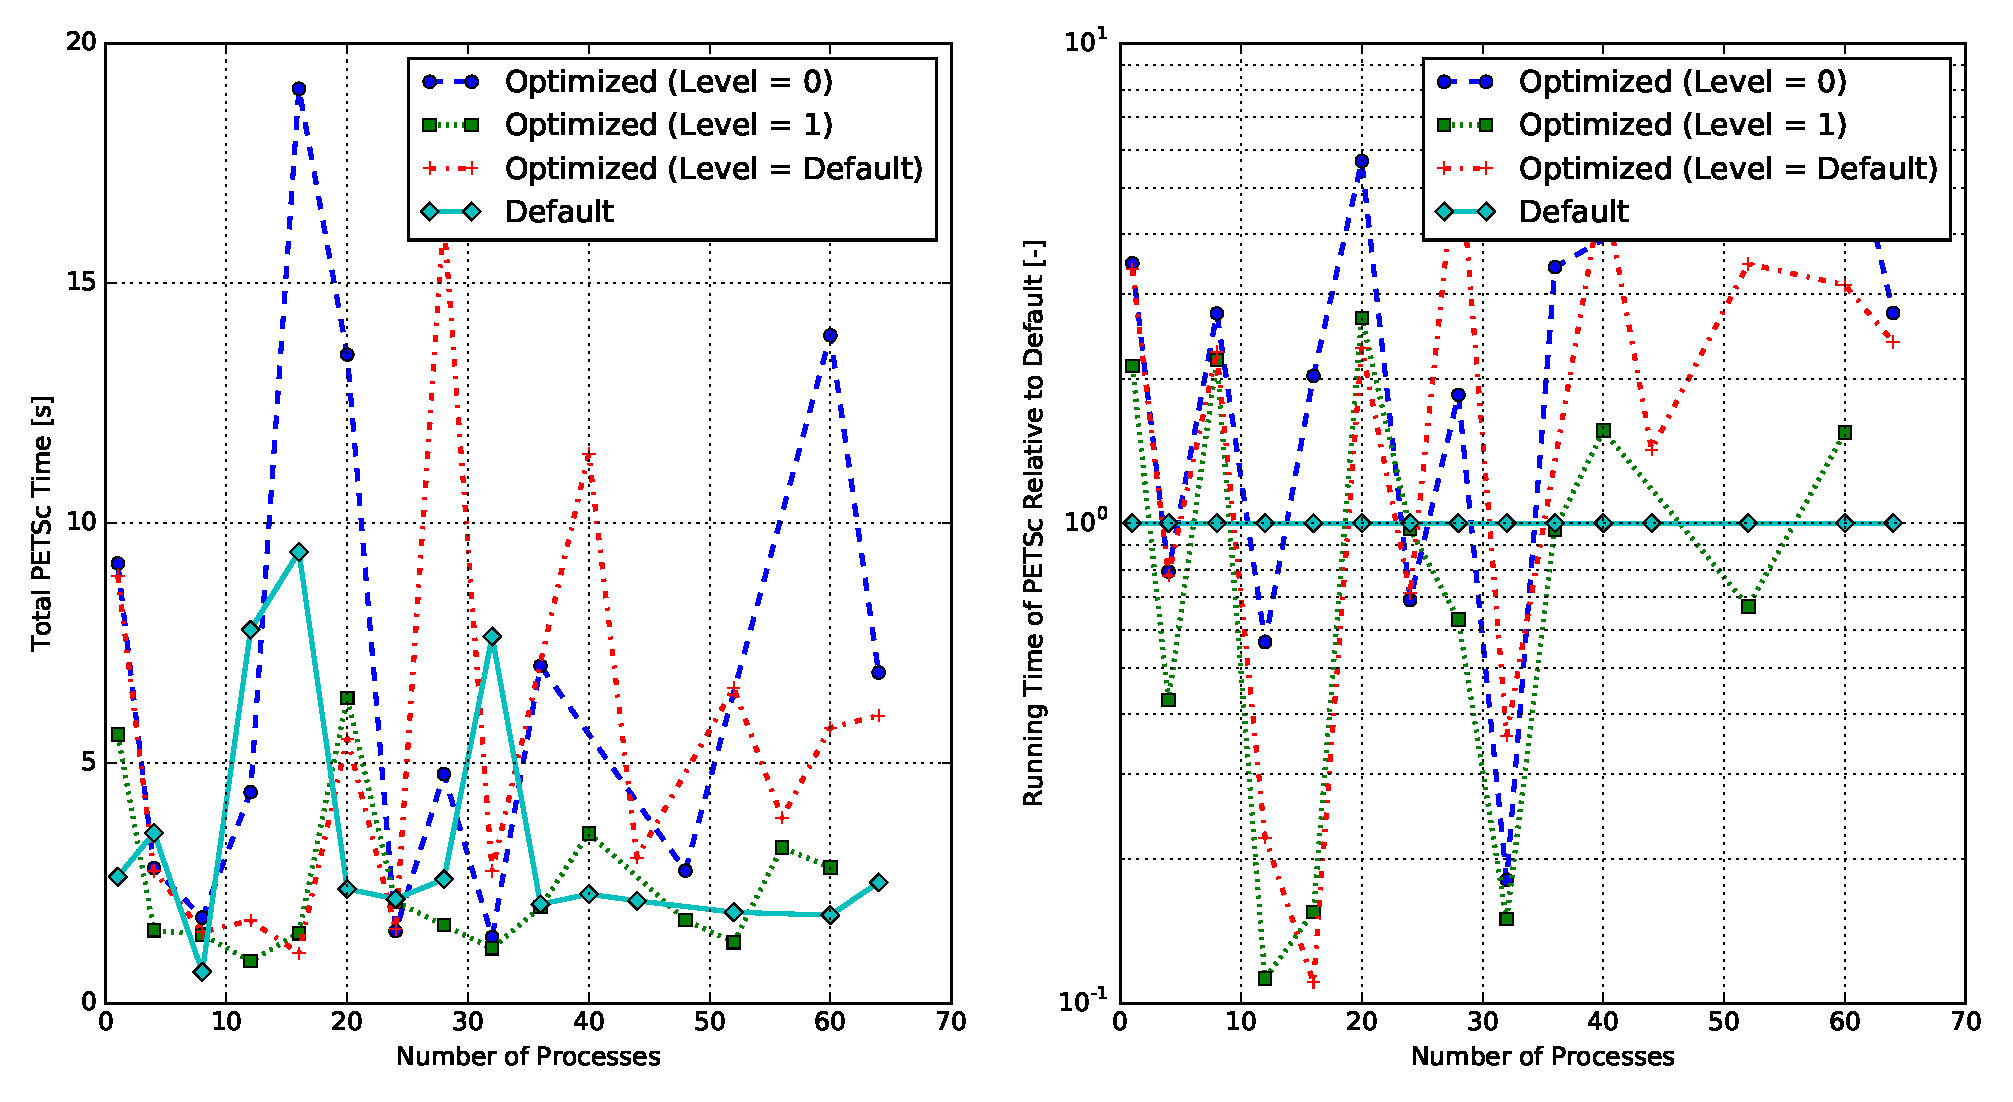
\includegraphics[width=\textwidth]{FIGURES/petsc-optimization/256x64-laminar.eps}
  \caption{Scaling test for the laminar case on a $256 \times 64$ grid}
  \label{fig:petsc-opt-scaling-laminar-256}
\end{figure}

\begin{figure}[h]
  \centering
  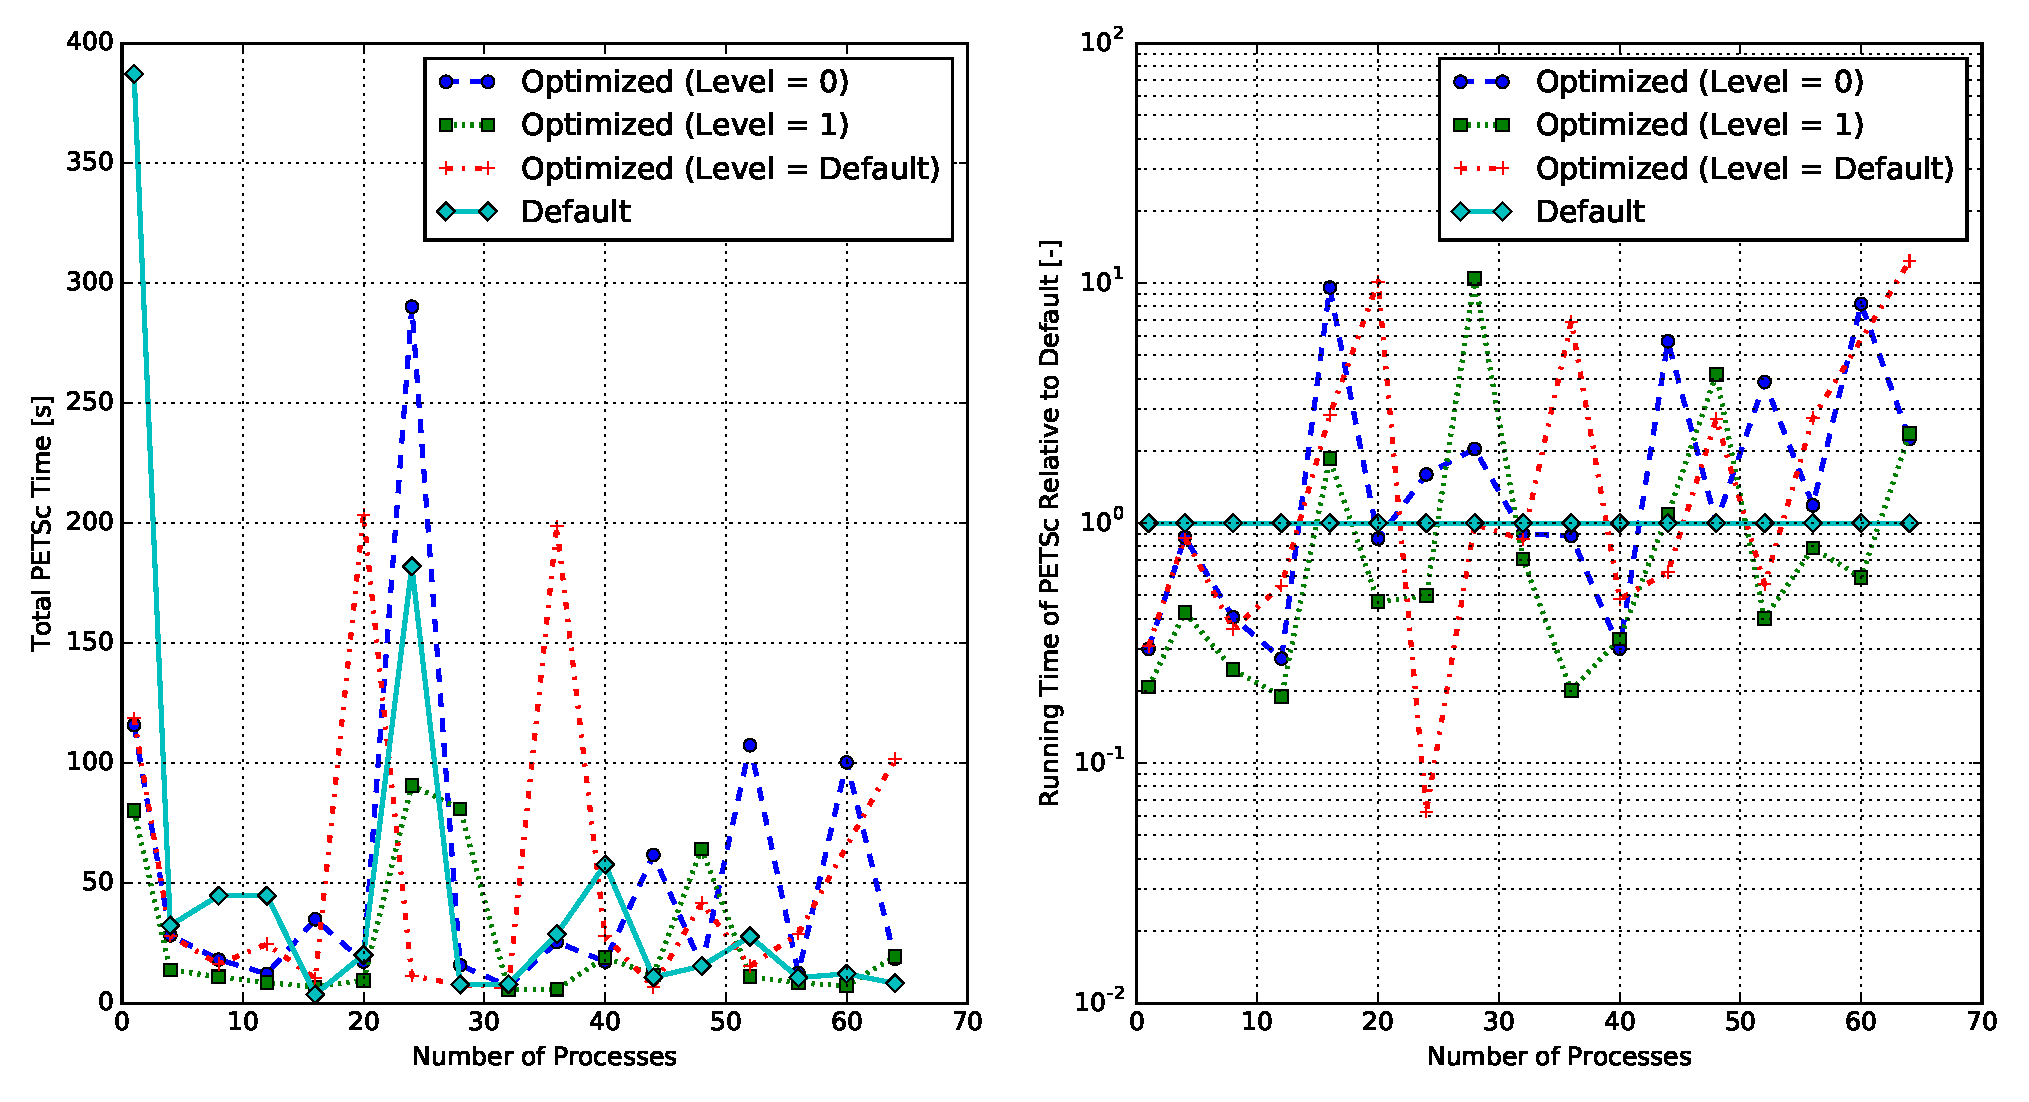
\includegraphics[width=\textwidth]{FIGURES/petsc-optimization/512x128-laminar.eps}
  \caption{Scaling test for the laminar case on a $512 \times 128$ grid}
  \label{fig:petsc-opt-scaling-laminar-512}
\end{figure}

\begin{figure}[h]
  \centering
  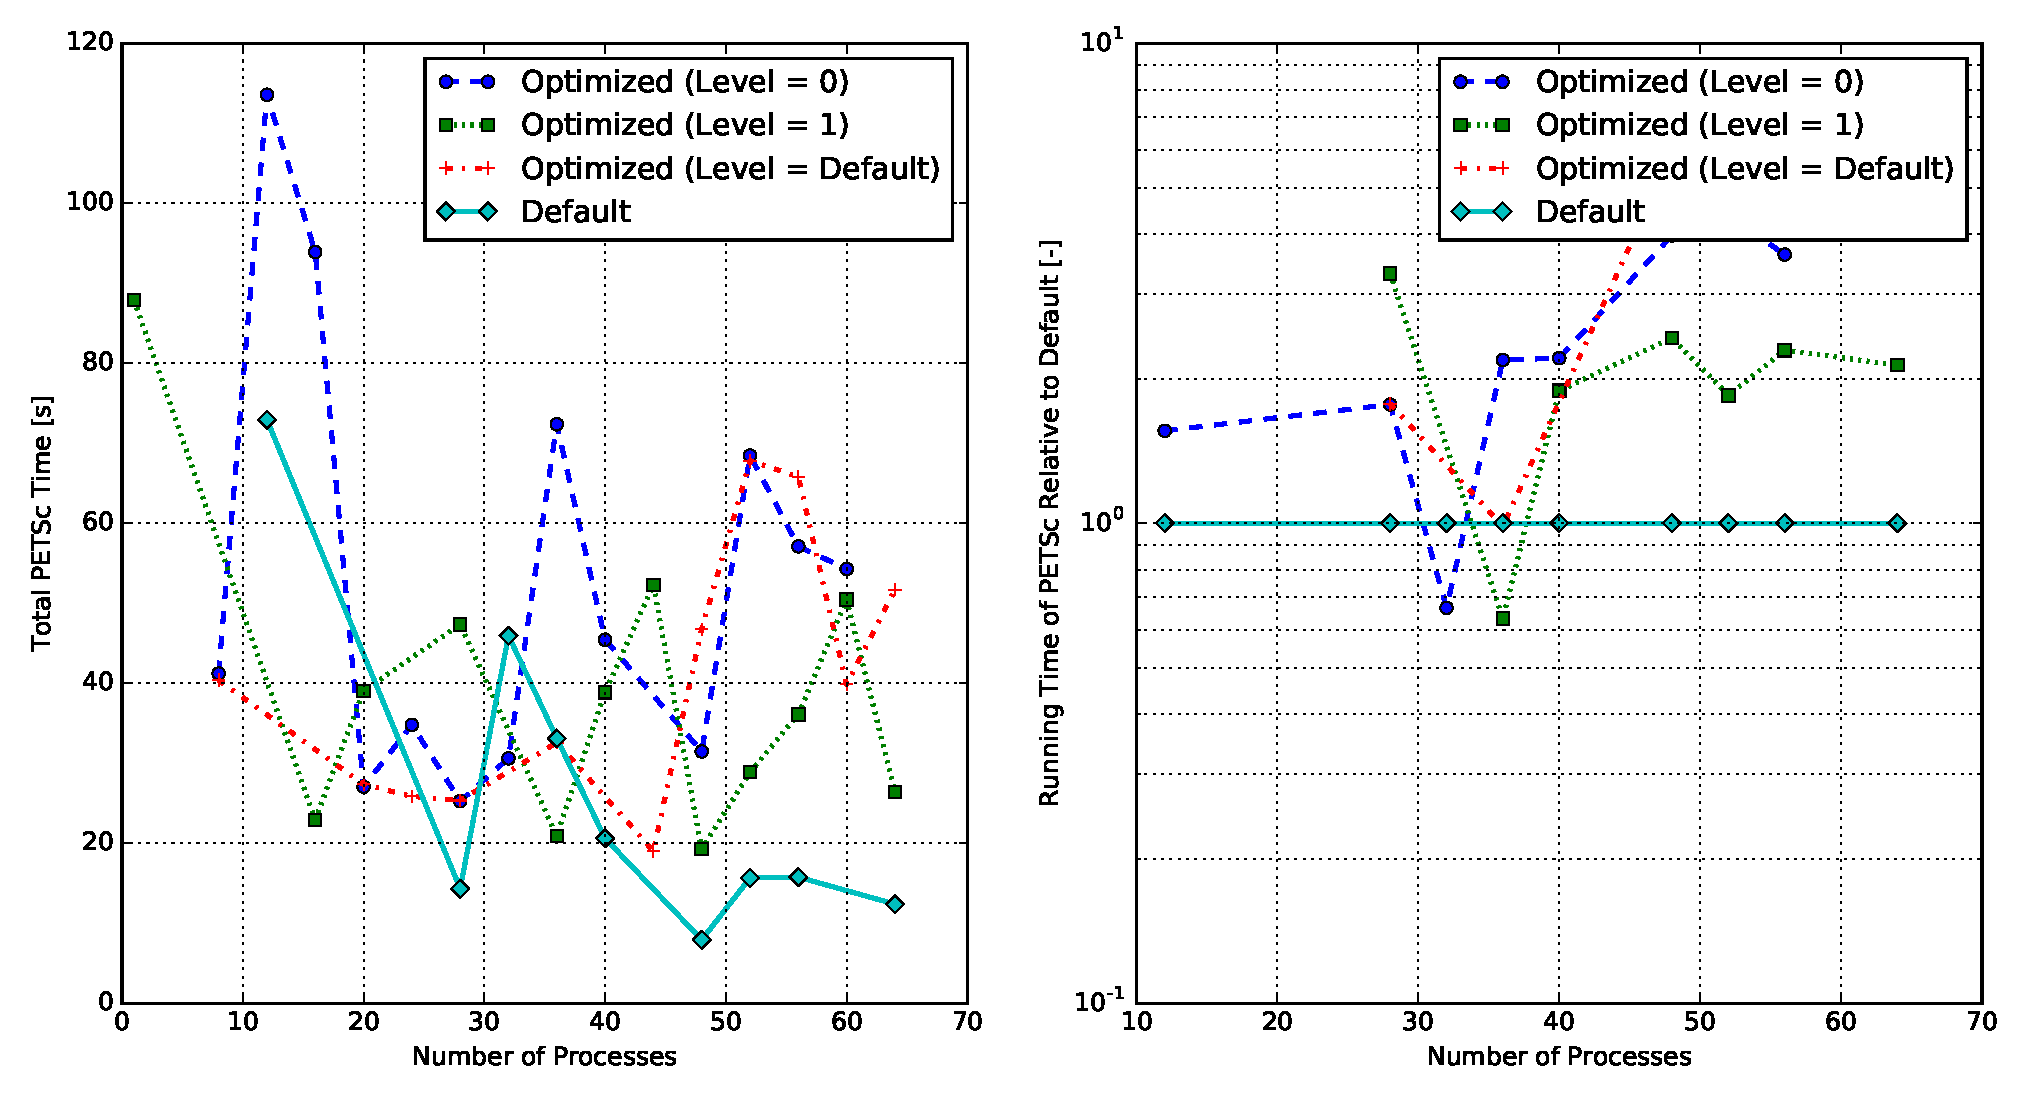
\includegraphics[width=\textwidth]{FIGURES/petsc-optimization/256x64-algebraic.eps}
  \caption{Scaling test for the algebraic case on a $256 \times 64$ grid}
  \label{fig:petsc-opt-scaling-algebraic-256}
\end{figure}

\begin{figure}[h]
  \centering
  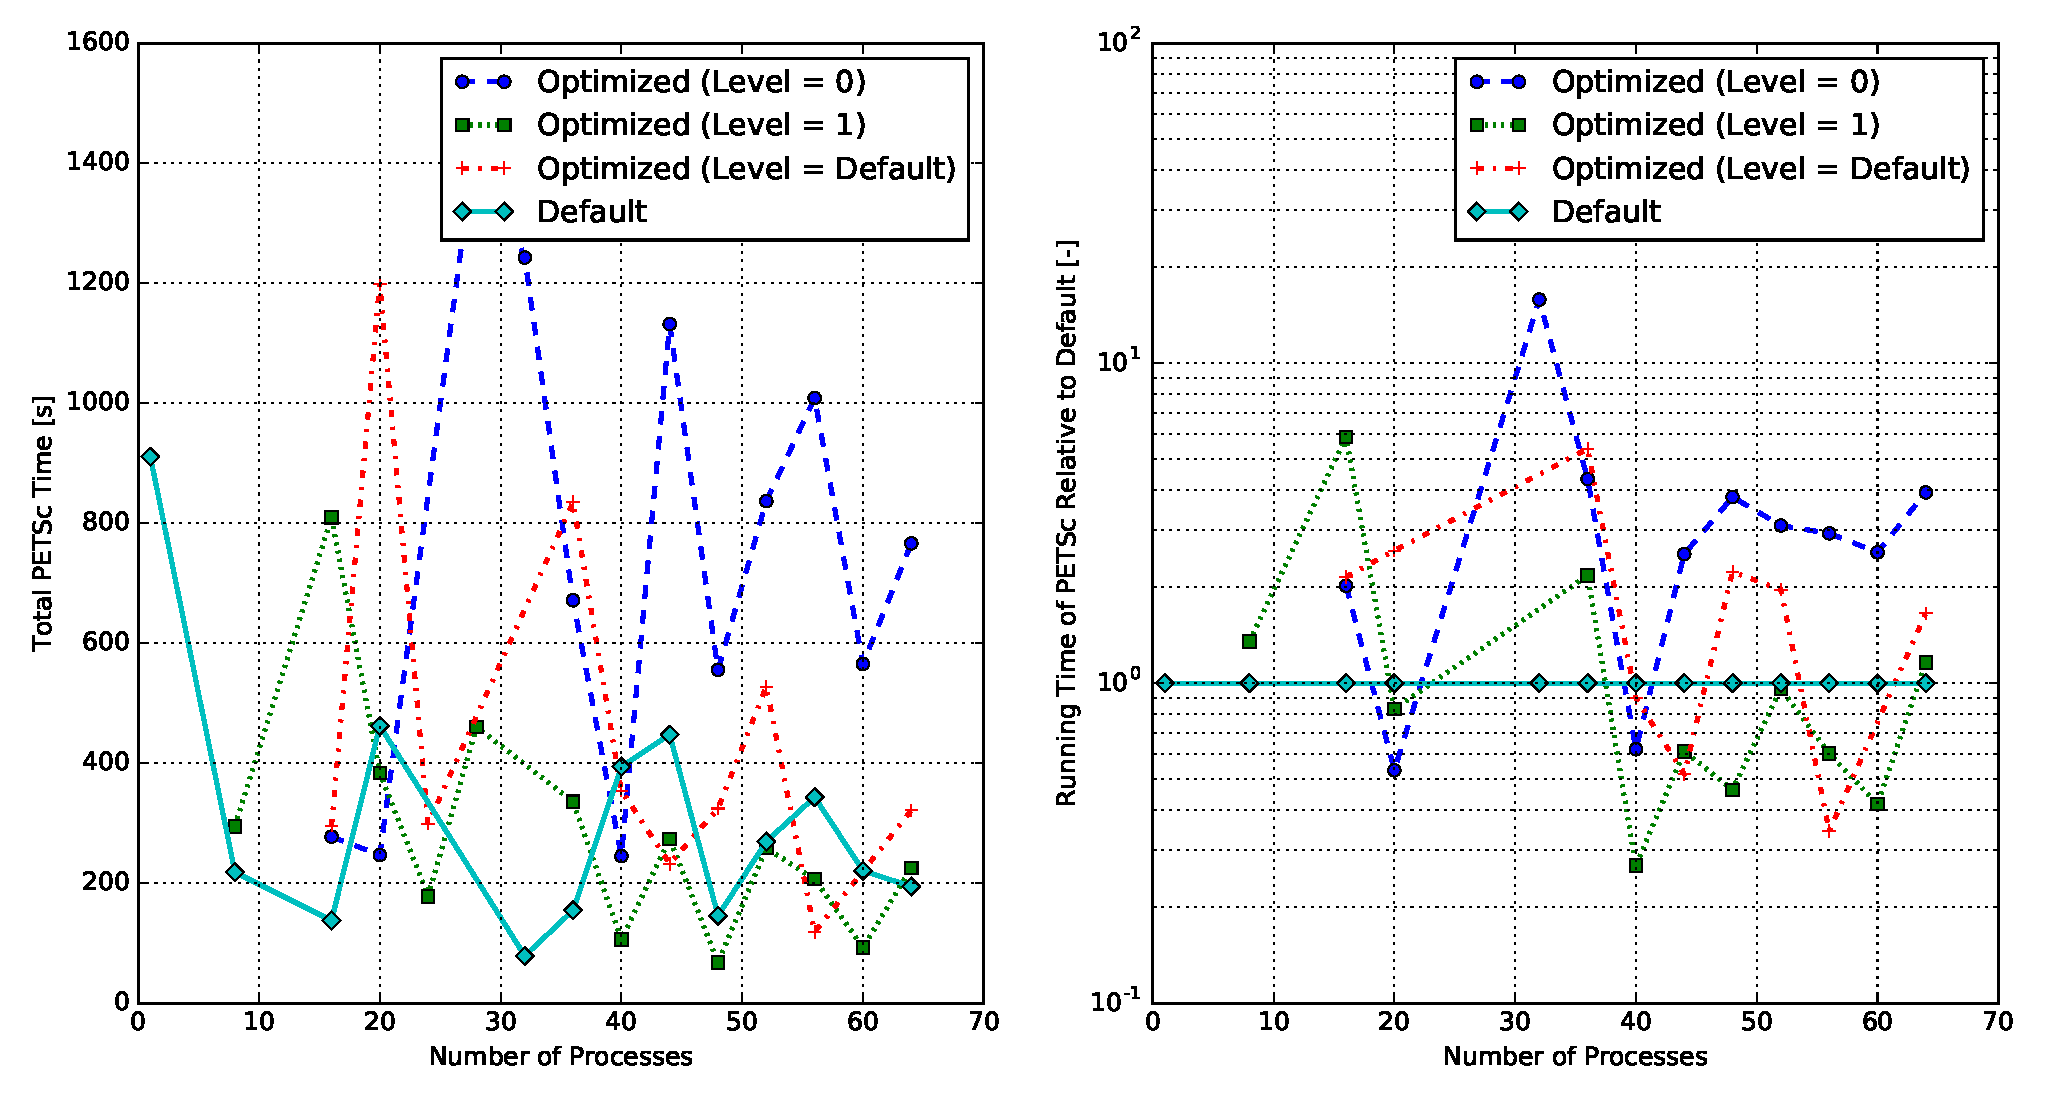
\includegraphics[width=\textwidth]{FIGURES/petsc-optimization/512x128-algebraic.eps}
  \caption{Scaling test for the algebraic case on a $512 \times 128$ grid}
  \label{fig:petsc-opt-scaling-algebraic-512}
\end{figure}

% chapter performance_tests (end)
